\documentclass{beamer}

\pdfmapfile{+sansmathaccent.map}


\mode<presentation>
{
	\usetheme{Warsaw} % or try Darmstadt, Madrid, Warsaw, Rochester, CambridgeUS, ...
	\usecolortheme{seahorse} % or try seahorse, beaver, crane, wolverine, ...
	\usefonttheme{serif}  % or try serif, structurebold, ...
	\setbeamertemplate{navigation symbols}{}
	\setbeamertemplate{caption}[numbered]
} 


%%%%%%%%%%%%%%%%%%%%%%%%%%%%
% itemize settings


%%%%%%%%%%%%%%%%%%%%%%%%%%%%
% itemize settings

\definecolor{myhotpink}{RGB}{255, 80, 200}
\definecolor{mywarmpink}{RGB}{255, 60, 160}
\definecolor{mylightpink}{RGB}{255, 80, 200}
\definecolor{mypink}{RGB}{255, 30, 80}
\definecolor{mydarkpink}{RGB}{155, 25, 60}

\definecolor{mypaleblue}{RGB}{240, 240, 255}
\definecolor{mylightblue}{RGB}{120, 150, 255}
\definecolor{myblue}{RGB}{90, 90, 255}
\definecolor{mygblue}{RGB}{70, 110, 240}
\definecolor{mycourseblue}{RGB}{120, 140, 255}
\definecolor{mycourselightblue}{RGB}{245, 250, 255}
\definecolor{mydarkblue}{RGB}{0, 0, 180}
\definecolor{myblackblue}{RGB}{40, 40, 120}

\definecolor{mygreen}{RGB}{0, 200, 0}
\definecolor{mygreen2}{RGB}{245, 255, 230}
\definecolor{mydarkgreen}{RGB}{0, 120, 0}
\definecolor{mydarkgreen}{RGB}{0, 120, 0}


\definecolor{mygray}{gray}{0.8}
\definecolor{mydarkgray}{RGB}{80, 80, 160}
\definecolor{mylightgray}{RGB}{160, 160, 160}

\definecolor{mydarkred}{RGB}{160, 30, 30}
\definecolor{mylightred}{RGB}{255, 150, 150}
\definecolor{myred}{RGB}{200, 110, 110}
\definecolor{myblackred}{RGB}{120, 40, 40}

\definecolor{mypink}{RGB}{255, 30, 80}
\definecolor{myhotpink}{RGB}{255, 80, 200}
\definecolor{mywarmpink}{RGB}{255, 60, 160}
\definecolor{mylightpink}{RGB}{255, 80, 200}
\definecolor{mydarkpink}{RGB}{155, 25, 60}
\definecolor{mywhitepink}{RGB}{255, 240, 240}

\definecolor{mydarkcolor}{RGB}{60, 25, 155}
\definecolor{mylightcolor}{RGB}{130, 180, 250}



\setbeamertemplate{itemize items}[default]

\setbeamertemplate{itemize item}{\color{myblackblue}$\blacksquare$}
\setbeamertemplate{itemize subitem}{\color{mygblue}$\blacktriangleright$}
\setbeamertemplate{itemize subsubitem}{\color{mygray}$\blacksquare$}

\setbeamercolor{palette quaternary}{fg=white,bg=mycourseblue}
\setbeamercolor{titlelike}{parent=palette quaternary}

\setbeamercolor{palette quaternary2}{fg=black,bg=mycourselightblue}
\setbeamercolor{frametitle}{parent=palette quaternary2}

\setbeamerfont{frametitle}{size=\Large,series=\scshape}
\setbeamerfont{framesubtitle}{size=\normalsize,series=\upshape}





%%%%%%%%%%%%%%%%%%%%%%%%%%%%
% block settings

\setbeamercolor{block title}{bg=red!30,fg=black}

\setbeamercolor*{block title example}{bg=mygreen!40!white,fg=black}

\setbeamercolor*{block body example}{fg= black, bg= mygreen2}


%%%%%%%%%%%%%%%%%%%%%%%%%%%%
% URL settings
\hypersetup{
	colorlinks=true,
	linkcolor=blue,
	filecolor=blue,      
	urlcolor=blue,
}

%%%%%%%%%%%%%%%%%%%%%%%%%%

\renewcommand{\familydefault}{\rmdefault}


\newcommand{\mycolor}[1] {
\setbeamercolor{normal text}{fg={#1}} % Recolors standard body text
\setbeamercolor{structure}{fg={#1}}   % Recolors bullets and structure items
\usebeamercolor[fg]{normal text}      % Applies the normal text color immediately
}


\usepackage{amsmath}
\usepackage{mathtools}

\usepackage{cancel}
\usepackage{centernot}

\usepackage{changepage}
\usepackage{subcaption}

\usepackage{qrcode}

\newcommand{\bo}[1] {\mathbf{#1}}
\newcommand{\R}{\mathbb{R}} 
\newcommand{\T}{^\top}     



\newcommand{\mydate}{Fall 2026}

\newcommand{\mygit}{\textcolor{blue}{\href{https://github.com/SergeiSa/Advanced-Control-2026}{github.com/SergeiSa/Advanced-Control-2026}}}

\newcommand{\myqr}{ \textcolor{black}{\qrcode[height=1.5in]{https://github.com/SergeiSa/Advanced-Control-2026}}
}

\newcommand{\myqrframe}{
	\begin{frame}
		\centerline{Lecture slides are available via Github:}
		\bigskip
		\centerline{\mygit}
		\bigskip
		\myqr
	\end{frame}
}


\newcommand{\bref}[2] {\textcolor{blue}{\href{#1}{#2}}}

%%%%%%%%%%%%%%%%%%%%%%%%%%%%
% code settings

\usepackage{listings}
\usepackage{color}
% \definecolor{mygreen}{rgb}{0,0.6,0}
% \definecolor{mygray}{rgb}{0.5,0.5,0.5}
\definecolor{mymauve}{rgb}{0.58,0,0.82}
\lstset{ 
	backgroundcolor=\color{white},   % choose the background color; you must add \usepackage{color} or \usepackage{xcolor}; should come as last argument
	basicstyle=\footnotesize,        % the size of the fonts that are used for the code
	breakatwhitespace=false,         % sets if automatic breaks should only happen at whitespace
	breaklines=true,                 % sets automatic line breaking
	captionpos=b,                    % sets the caption-position to bottom
	commentstyle=\color{mygreen},    % comment style
	deletekeywords={...},            % if you want to delete keywords from the given language
	escapeinside={\%*}{*)},          % if you want to add LaTeX within your code
	extendedchars=true,              % lets you use non-ASCII characters; for 8-bits encodings only, does not work with UTF-8
	firstnumber=0000,                % start line enumeration with line 0000
	frame=single,	                   % adds a frame around the code
	keepspaces=true,                 % keeps spaces in text, useful for keeping indentation of code (possibly needs columns=flexible)
	keywordstyle=\color{blue},       % keyword style
	language=Octave,                 % the language of the code
	morekeywords={*,...},            % if you want to add more keywords to the set
	numbers=left,                    % where to put the line-numbers; possible values are (none, left, right)
	numbersep=5pt,                   % how far the line-numbers are from the code
	numberstyle=\tiny\color{mygray}, % the style that is used for the line-numbers
	rulecolor=\color{black},         % if not set, the frame-color may be changed on line-breaks within not-black text (e.g. comments (green here))
	showspaces=false,                % show spaces everywhere adding particular underscores; it overrides 'showstringspaces'
	showstringspaces=false,          % underline spaces within strings only
	showtabs=false,                  % show tabs within strings adding particular underscores
	stepnumber=2,                    % the step between two line-numbers. If it's 1, each line will be numbered
	stringstyle=\color{mymauve},     % string literal style
	tabsize=2,	                   % sets default tabsize to 2 spaces
	title=\lstname                   % show the filename of files included with \lstinputlisting; also try caption instead of title
}


%%%%%%%%%%%%%%%%%%%%%%%%%%%%
% URL settings
\hypersetup{
	colorlinks=false,
	linkcolor=blue,
	filecolor=blue,      
	urlcolor=blue,
}

%%%%%%%%%%%%%%%%%%%%%%%%%%

%%%%%%%%%%%%%%%%%%%%%%%%%%%%
% tikz settings

\usepackage{tikz}
\tikzset{every picture/.style={line width=0.75pt}}
\usetikzlibrary{shapes.geometric, decorations.markings, positioning, patterns, calc, arrows.meta}


\title{Trajectory Planning}
\subtitle{Advanced Control}
\author{by Sergei Savin}
\centering
\date{\mydate}



\begin{document}
\maketitle


\begin{frame}{Content}
	\begin{itemize}
		\item Stability and Trajectory Planning
		\item Trajectory planning -- illustration
		\item Example: Inverted pendulum swing up
		\item Example: Cart-Pole
		\item Path vs.\ Trajectory
		\item Feasible Trajectory
		\item Trajectory Optimization
		\item Direct Shooting
		\item Parameterizing the Control Input
		\item Solving Direct Shooting
		\item Literature
	\end{itemize}
\end{frame}


\begin{frame}{Stability and Trajectory Planning}
	\begin{flushleft}
	
	For a dynamical system
	\[
	\dot{x}=f(x,u),
	\]
	we can consider two different tasks:
	
	\begin{enumerate}
		\item Find a control law that takes the system
		from an initial state $x_A$ to a desired state $x_B$.
		
		\item Find a control law that makes the system
		stay near $x_B$ (or converge to it) once it has
		arrived sufficiently close.
	\end{enumerate}
	
	\vspace{0.5em}
	
	The second problem is the problem of
	\textbf{stabilizing control}.
	
	The first problem is the problem of
	\textbf{trajectory planning}.
	
	\end{flushleft}
\end{frame}


\begin{frame}{Trajectory planning - illustration}
	\begin{flushleft}
		
			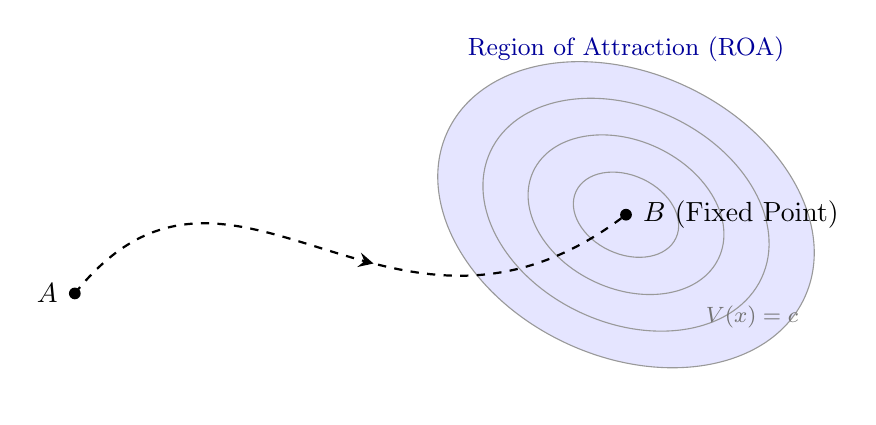
\begin{tikzpicture}[
		% Arrow decoration for the trajectory path
		path arrow/.style={
			postaction={
				decorate,
				decoration={
					markings,
					mark=at position 0.55 with {\arrow[scale=1.3]{stealth}}
				}
			}
		},
		% Point marker style
		point/.style={
			circle,
			fill=black,
			inner sep=1.5pt
		}
		]
		
		% Define coordinates
		\coordinate (A) at (-4, -0.5);
		\coordinate (B) at (3, 0.5);
		
		% --- Region of Attraction (ROA) Fill ---
		% Fills the outer ellipsoid around point B
		\fill[blue!10, rotate around={-25:(B)}] (B) ellipse (2.5cm and 1.8cm);
		
		% --- Lyapunov Function Ellipsoids (Contours) ---
		% Diminishing sizes around point B
		\begin{scope}[rotate around={-25:(B)}]
			\draw[thin, color=gray!80] (B) ellipse (2.5cm and 1.8cm);
			\draw[thin, color=gray!80] (B) ellipse (1.9cm and 1.37cm);
			\draw[thin, color=gray!80] (B) ellipse (1.3cm and 0.94cm);
			\draw[thin, color=gray!80] (B) ellipse (0.7cm and 0.5cm);
		\end{scope}
		
		% --- Trajectory Path ---
		% Smooth curved path from A into B
		\draw[thick, dashed, path arrow] 
		(A) .. controls (-2, 2) and (0, -1.8) .. (B);
		
		% --- Points and Labels ---
		\node[point, label=left:{$A$}] at (A) {};
		\node[point, label=right:{$B$ (Fixed Point)}] at (B) {};
		
		% --- Optional Labels ---
		\node[blue!60!black, font=\small] at ($(B) + (0, 2.1)$) {Region of Attraction (ROA)};
		\node[gray!90!black, font=\footnotesize] at ($(B) + (1.6, -1.3)$) {$V(x) = c$};
		
	\end{tikzpicture}
		
	\end{flushleft}
\end{frame}


\begin{frame}{Example Inverted pendulum swing up}
	\begin{flushleft}
		
		
\begin{center}
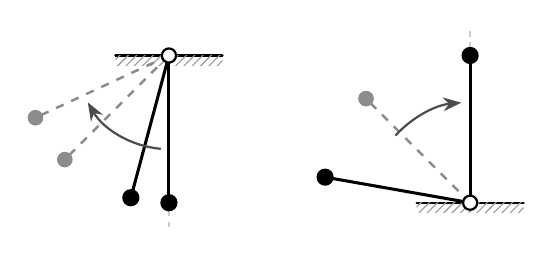
\begin{tikzpicture}[
	scale=0.85,
	>=Stealth,
	base/.style={thick, line cap=round},
	stable/.style={draw=black, line width=1.1pt},
	intermediate/.style={draw=black!45, line width=0.9pt, dashed},
	pivot/.style={fill=white, draw=black, thick},
	bob/.style={circle, fill=black, inner sep=2.2pt},
	bob gray/.style={circle, fill=black!45, inner sep=2pt},
	arc arrow/.style={->, draw=black!70, thick, >=Stealth}
	]
	
	\def\L{2.2} % Length of pendulum arm
	
	% --- LEFT SIDE: LOWER EQUILIBRIUM ---
	\coordinate (O1) at (0, 0);
	
	% Base Mount
	\draw[base] (-0.8,0) -- (0.8,0);
	\fill[pattern=north east lines, pattern color=black!40] (-0.8,-0.15) rectangle (0.8,0);
	
	% Ground / Reference dashed line
	\draw[gray!40, dash pattern=on 2pt off 2pt] (O1) -- ++(0, -\L - 0.4);
	
	% 4 States
	\draw[stable] (O1) -- ++(270:\L) node[bob] {};
	\draw[stable] (O1) -- ++(255:\L) node[bob] {};
	\draw[intermediate] (O1) -- ++(225:\L) node[bob gray] {};
	\draw[intermediate] (O1) -- ++(205:\L) node[bob gray] {};
	
	% Pivot Joint
	\draw[pivot] (O1) circle (3pt);
	
	% Arc Arrow
	\draw[arc arrow] (265:1.4) arc (265:210:1.4);
	
	
	% --- RIGHT SIDE: UPPER EQUILIBRIUM (Shifted down to align top-to-top) ---
	% Offset y by -\L so the top of the 180-deg pendulum reaches y = 0
	\coordinate (O2) at (4.5, -\L);
	
	% Base Mount
	\draw[base] (O2) ++(-0.8,0) -- ++(1.6,0);
	\fill[pattern=north east lines, pattern color=black!40] (O2) ++(-0.8,-0.15) rectangle ++(1.6,0.15);
	
	% Vertical Reference line
	\draw[gray!40, dash pattern=on 2pt off 2pt] (O2) -- ++(0, \L + 0.4);
	
	% States
	\draw[intermediate] (O2) -- ++(135:\L) node[bob gray] {};
	\draw[stable] (O2) -- ++(170:\L) node[bob] {};
	\draw[stable] (O2) -- ++(90:\L) node[bob] {};
	
	% Pivot Joint
	\draw[pivot] (O2) circle (3pt);
	
	% Arc Arrow
	\draw[arc arrow] ($(O2)+(138:1.5)$) arc (138:95:1.5);
	
\end{tikzpicture}
\end{center}
		
		
		For a pendulum, we can consider two separate problems: 1) plan a trajectory that takes the pendulum from the lower equilibrium to the upper equilibrium; 2) find a control law that stabilizes the upper equilibrium.
		
		\bigskip
		
		The first problem can be challenging if the motor is weak
		and has a small torque limit. Instead of lifting the pendulum directly, we may need to
		\textbf{swing it up}.
		
	\end{flushleft}
\end{frame}




\begin{frame}{Example: Cart-Pole}
	\begin{flushleft}
	
	% TODO: \usepackage{graphicx} required
	\begin{figure}
		\centering
		\includegraphics[width=0.7\linewidth]{"cartpole swing up"}
		\label{fig:cartpole-swing-up}
	\end{figure}
	
	
	For a cart-pole, we can again consider two separate problems:1) plan a trajectory that takes the pole
		from the lower equilibrium to the upper equilibrium; 2) find a control law that stabilizes the upper equilibrium.
		
		\medskip
	
	There is no motor directly between the cart and the pole. Therefore, we cannot simply apply a torque: instead, we must move the cart so that its motion creates \textbf{inertial forces} that swing the pole upward.
	
	\end{flushleft}
\end{frame}


\begin{frame}{Path vs.\ Trajectory}
	\begin{flushleft}
	
	Consider two states $x_A$ and $x_B$. A curve connecting them in state space is called a
	\textbf{path}.
	
\bigskip
	
	A path tells us the sequence of states that the system should pass through, but does not specify \emph{when} those states should be reached.
	
	\bigskip
	
	A path together with its timing is called a	\textbf{trajectory}. We can denote it as $x(t)$.
	
	\end{flushleft}
\end{frame}


\begin{frame}{Feasible Trajectory}
	\begin{flushleft}
	
	Not every trajectory can actually be produced by a dynamical system. For a system with control input
	\[
	\dot{x}=f(x,u),
	\]
	a trajectory $x^*(t)$ is \emph{feasible} if there exists 	a control input $u^*(t)$ such that
	
	\[
	\dot{x}^*(t)
	=
	f\bigl(x^*(t),u^*(t)\bigr),
	\qquad
	\forall t\in[0,T].
	\]
	
	
	\bigskip
	
	\begin{center}
\fbox{The trajectory must satisfy the system dynamics.}
	\end{center}
	
	\end{flushleft}
\end{frame}



\begin{frame}{Trajectory Optimization}
	\begin{flushleft}
		Trajectory optimization is the problem of finding a
		\emph{feasible trajectory} that minimizes a chosen
		cost function.
		
		\vspace{0.5em}
		
		For example, we can formulate the problem as
		\[
		\begin{aligned}
			\min_{x(t),u(t),T}\quad
			&
			\Phi\bigl(x(T)\bigr)
			+
			\int_0^T L\bigl(x(t),u(t)\bigr)\,dt
			\\
			\text{s.t.}\quad
			&
			\dot{x}(t)=f\bigl(x(t),u(t)\bigr),
			\\
			&
			x(0)=x_A,
			\qquad
			x(T)=x_B.
		\end{aligned}
		\]
		
		\begin{itemize}
			\item $\Phi(x(T))$ is the \textbf{terminal cost}, which
			penalizes the final state.
			
			\item $L(x(t),u(t))$ is the \textbf{running cost}, which
			penalizes the state and control along the trajectory.
		\end{itemize}
		
		The particular choice of $\Phi$ and $L$ depends on what
		we want the trajectory to achieve.
	\end{flushleft}
\end{frame}

\begin{frame}{Direct Shooting}
	\begin{flushleft}
		Observe that, for a given control input $u(t)$ and
		initial condition $x(0)=x_0$, the resulting trajectory is completely determined by
		the system dynamics
		\[
		\dot{x}=f(x,u).
		\]
		
		\vspace{0.5em}
		
		Therefore, we do not have to choose both $u(t)$ and $x(t)$.
		
		Instead, we can:
		\begin{itemize}
			\item choose $u(t)$;
			\item simulate the system forward to obtain $x(t)$.
		\end{itemize}
		
		\vspace{0.5em}
		
		This approach to trajectory optimization is called
		\textbf{direct shooting}.
	\end{flushleft}
\end{frame}


\begin{frame}{Parameterizing the Control Input}
	\begin{flushleft}
		There are multiple ways to parameterize $u(t)$ for
		direct shooting.
		
		\begin{itemize}
			\item Piecewise constant:
			\[
			u(t)=u_i,
			\qquad
			t\in[t_i,t_{i+1}).
			\]
			
			\item Higher-order polynomials on each time interval.
			
			\item Splines.
			
			\item A single time-dependent function, e.g.:
			\[
			u(t)=c_0+c_1t+c_2t^2+c_3t^3.
			\]
		\end{itemize}
		
		\vspace{0.5em}
		
		The key idea is to parameterize the control input using
		a finite number of parameters $c$:
		\[
		u(t)=u(c,t).
		\]
		
		The parameters $c$ then become the
		\textbf{decision variables} of the optimization problem.
	\end{flushleft}
\end{frame}


\begin{frame}{Solving Direct Shooting}
	\begin{flushleft}
		After parameterizing the control input as
		\[
		u(t)=u(c,t),
		\]
		the trajectory optimization problem becomes an optimization
		problem over the finite-dimensional vector $c$.
		
		\vspace{0.5em}
		
		An illuminating (although incomplete) picture of the
		optimization process is:
		
		\begin{enumerate}
			\item Given the current estimate of $c$, construct
			$u(c,t)$.
			
			\item Solve $\dot{x}=f(x,u(c,t))$ forward in time.
			
			\item Evaluate the cost and its gradient $J(c),
			\quad
			\nabla_c J(c)$.
			
			\item Update $c$ in a direction that decreases the cost.
			
			\item Repeat until convergence.
		\end{enumerate}
		
		\vspace{0.5em}
		
		This produces a trajectory $x(t)$ and control input $u(t)$
		that approximately solve the trajectory optimization problem.
	\end{flushleft}
\end{frame}

\begin{frame}{Literature}
	
	\begin{itemize}
		
		
		\item Russ Tedrake -- MIT:
		\bref{https://underactuated.mit.edu/trajopt.html}
		{Underactuated Robotics: Trajectory Optimization, ch. 10.}
		
	\end{itemize}
	
\end{frame}



\myqrframe




\end{document}
